% !TEX root=/home/tavant/these/manuscript/src/manuscript.tex

\section{Elements of the 2D PIC-MCC simulations}

  \subsection{Principe of the PIC simulations}

    The \ac{PIC} simulation models the movement of particles on a fixed grid.

    The grid is used to compute the electric field, in the electrostatic approximation by solving the Poisson equation

    \begin{equation}
      \label{eq-poisson}
      \Delta \phi = - \frac{\rho}{\epsilon_0}
    \end{equation}

    where $\phi$ is the electric potential, $\rho$ is the charge density, and $\epsilon_0$ the vacuum permittivity, or the Maxwell equations.

    The charge density $\rho$ is computed by depositing the particle over the cells, using the usual Cloud-in-cell model \cite{birdsall1991}.

    The particles moves following the Lorenz forces
    \begin{equation}
      \label{eq-Lor}
      m \vec{a} = q E + q \vec{v} \times \vec{B}
    \end{equation}
    with $m$ and $q$ the particle mass and electric charge respectively.
    The numerical particles followed in the simulations correspond to $q_f$ physical particles, with
    \begin{equation}
      q_f = \frac{n V}{\Npc}
    \end{equation}
    with $n$ the particle density, $V$ the volume of a cell, and $\Npc$ the number of numerical particle in a cell.
    A large enough number of particle is needed in order to obtain physical results.
    Indeed, insufficient number of particles leads to numerical heating \cite{ueda1994}.
    Usually, a minimum of 100 particles per cell are used, but recent results seem to encourage to use more particle \cite{janhunen2018}.

  \subsection{Monte Carlo collisions}

    In \ac{PIC} simulations, collisions between charged and neutral particles can be modeled by binary collision, but this approach is computationally costly.
    Instead, a Monte-Carlo algorithm can be used \cite{vahedi1995}.
    This approach is very efficient, and allow scattering, momentum transfer and ionization to be consistently model.

    The propellant used in \ac{HET} usually is \ac{Xe}, even if the recent constellation Starlink uses \ac{Kr}.
    The cross sections used for modeling \ac{Xe} or other gases collisions are taken from the {\sc LXCat} database project \cite{LXCat_web}.

    Except is other with stated, the elastic, inelastic scattering and ionization reactions listed in \cref{tab-reactXe} are used.
    The cross section values are summarised in \cref{fig-xexsection}.

    \begin{table}[hbtp]
      \centering
      \caption{Reactions used in the PIC simulations}
      \label{tab-reactXe}
      \begin{tabular}{ccc}
        Reaction & Threshold & Reference\\
        {\it Elastic scattering} & &\\
        e + Xe = e + Xe   & --   & \cite{Lxcat_Xe,Lxcat_Xe2} \\
        {\it Excitation} & &\\
        e + Xe = e + Xe$^*$   & 8.315eV   & \cite{Lxcat_Xe,Lxcat_Xe2} \\
        e + Xe = e + Xe$^*$   & 9.447eV   & \cite{Lxcat_Xe,Lxcat_Xe2} \\
        e + Xe = e + Xe$^*$   & 9.917eV   & \cite{Lxcat_Xe,Lxcat_Xe2} \\
        e + Xe = e + Xe$^*$   & 11.7eV    & \cite{Lxcat_Xe,Lxcat_Xe2} \\
        {\it Ionization} & &\\
        e + Xe = e + Xe$^+$   & 8.315eV   & \cite{Lxcat_Xe,Lxcat_Xe2} \\

      \end{tabular}

    \end{table}


    \begin{figure}[hbtp]
      \centering
      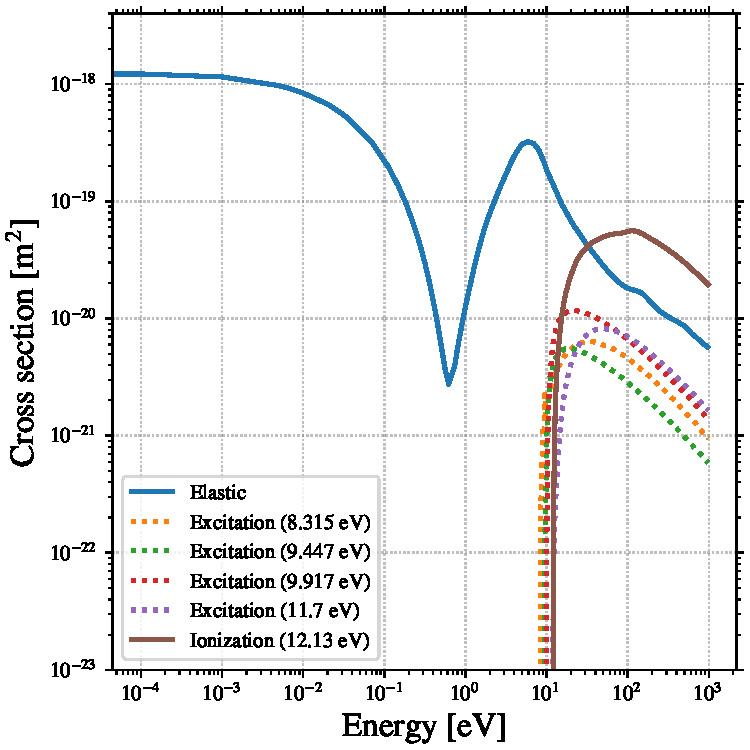
\includegraphics[width=\defaultwidth]{figure/xenon_cross_section.pdf}
      \caption{Cross section values used in the Monte Carlo procedure \cite{Lxcat_Xe,Lxcat_Xe2}.}
      \label{fig-xexsection}
    \end{figure}


\section{Numerical implementation of the Particle in cell simulation}

  \LPPic is an explicit electrostatic \ac{PIC} code.

  Every time-steps, the simulation loop presented in \cref{fig-picloop} is computed.

  \begin{figure}[hbtp]
    \centering
    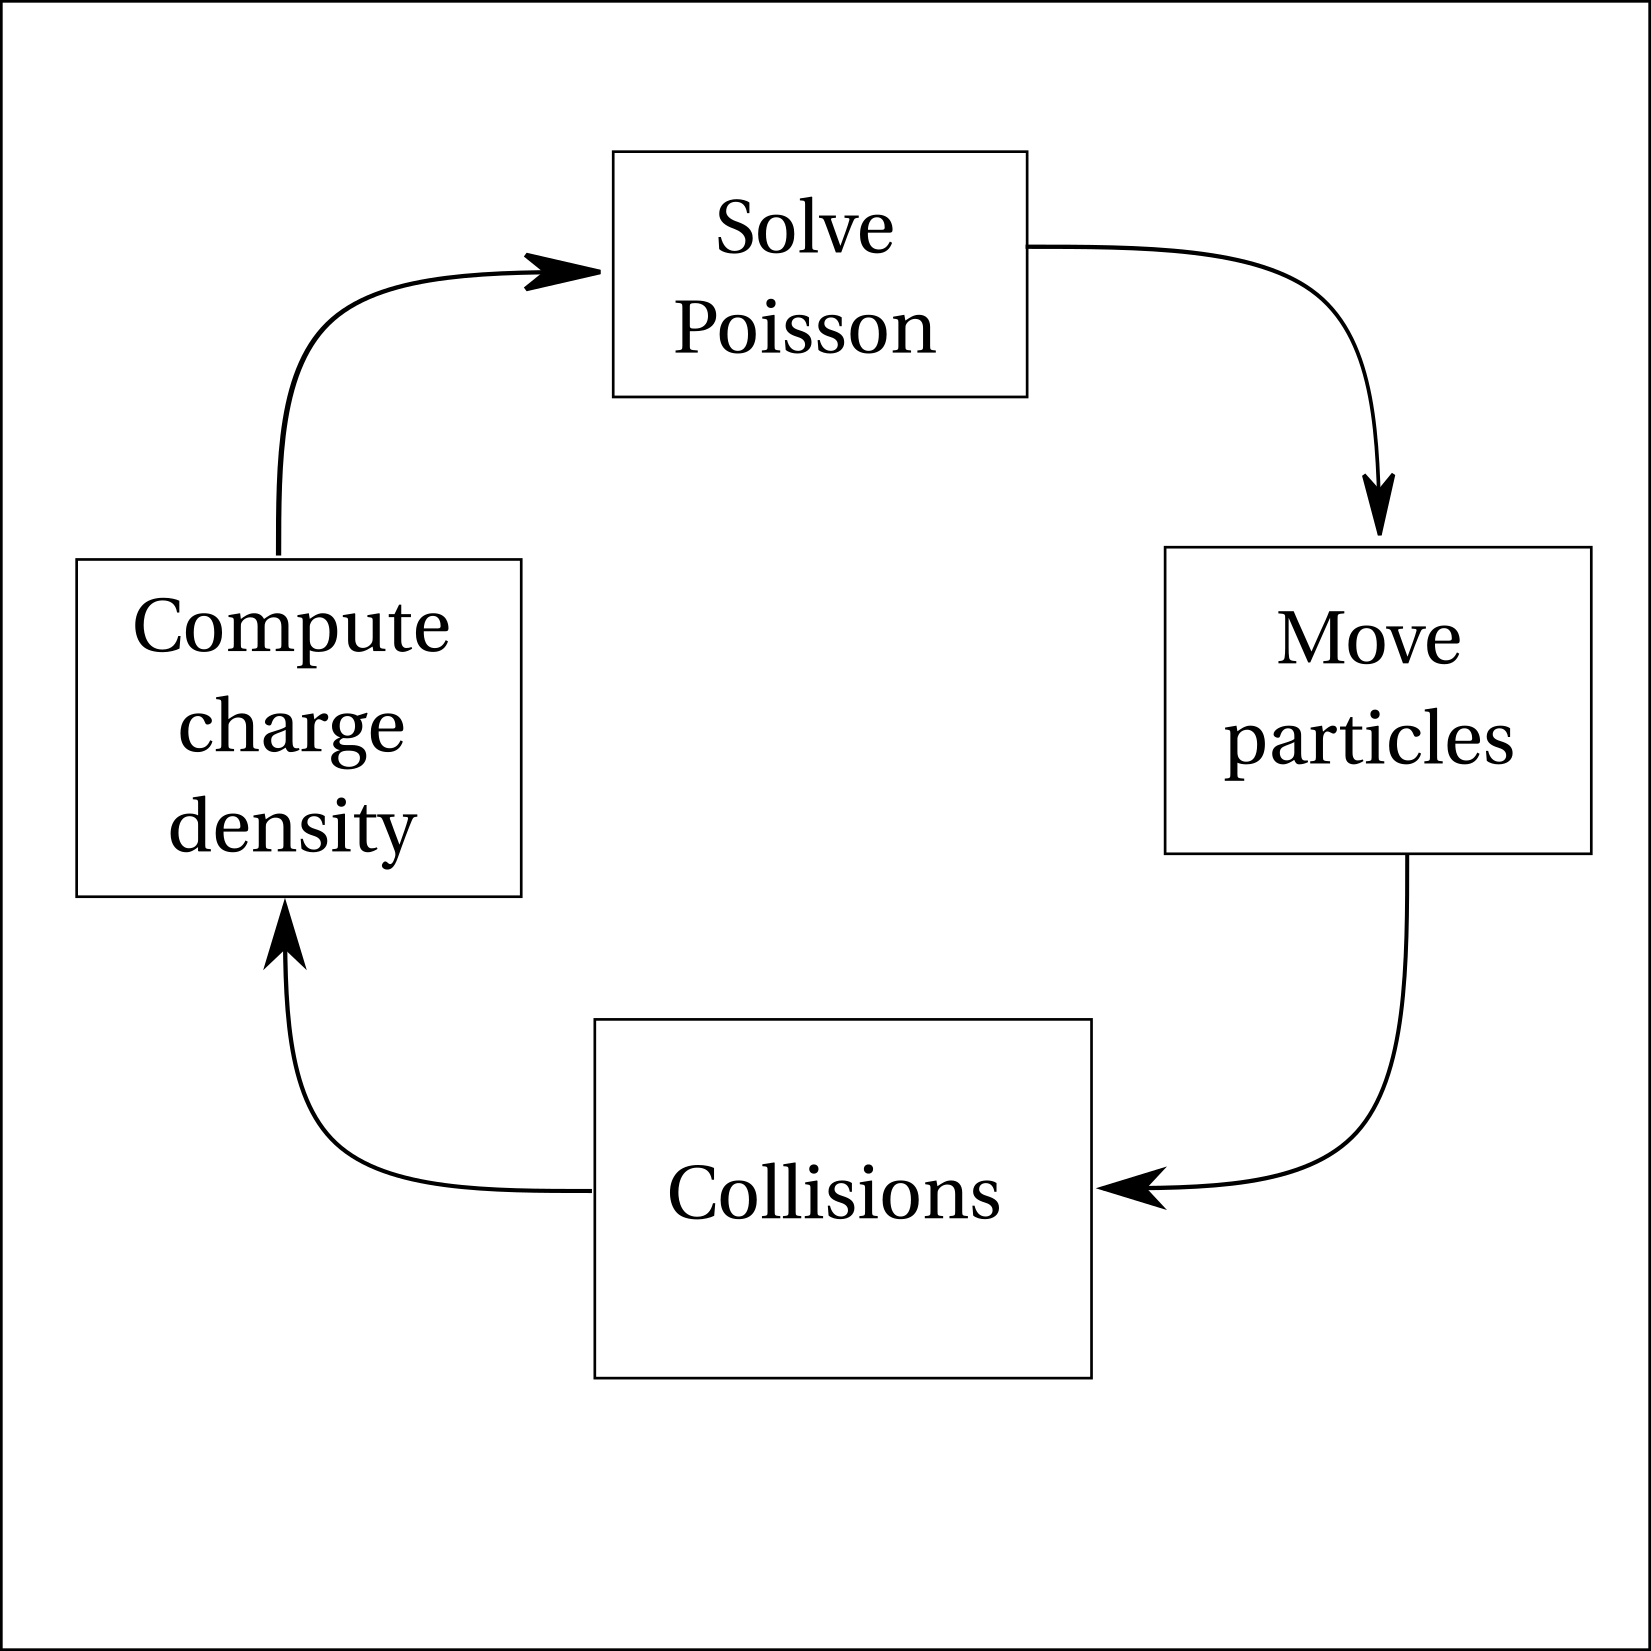
\includegraphics{picloop.png}
    \caption{\ac{PIC}-\ac{MCC} loop executed every time steps.}
    \label{fig-picloop}
  \end{figure}

  \subsection{Data used}
    In the \ac{PIC} simulation, there is two kind of data used:
    \begin{itemize}
      \item Particles
      \item Mesh
    \end{itemize}

    \paragraph{Particles}
    For each particles, are known its position $\vec{x}$ and its velocity $\vec{v}$.
    We can decouple the number of dimensions used for the velocity and the position.
    In most \ac{PIC}-\ac{MCC} simulations, the 3 directions of the velocity vector are followed in order to in order to take into account scattering.
    It is abbreviated as \acs{3V}.

    The dimension of the position depends of the dimension of the simulation domain, hence the mesh dimension.
    It is usual to find \acs{2D}\ac{3V} \ac{PIC} simulations, for particles with 3 directions on the velocity but 2 dimension in space.

    \subsection{Particle pusher}
    Integrating the movement equation \cref{eq-Lor} is deferent for magnetized and non-magnetized particles.

    For non-magnetized particles, we use \cite{birdsall1991} the leapfrog scheme
    \begin{align}\label{eq-leapfrog}
      v^t &= v^{t-1} + \frac{q}{m} E \dt, \\
      x^t &= x^{t-1} + v^t \dt,
    \end{align}
    with the superscript $t$ designing the time step, $q$ and $m$ the particle electric charge and mass, $E$ the electric field at the particle position, and \dt the time step duration.

    It is important to note that the leapfrog induces a shift of $\frac{\dt}{2}$ between the position and the velocity, as illustrated in \cref{fig-leapfrog}.
    \begin{figure}[hbtp]
      \centering
      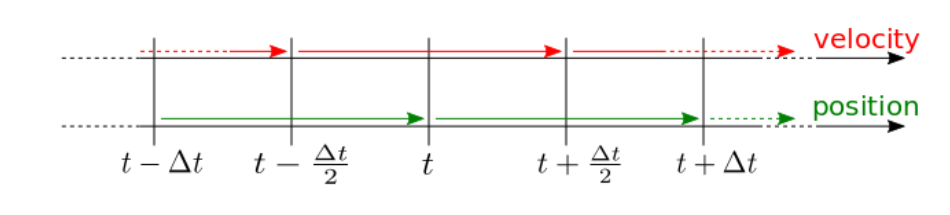
\includegraphics[width=\defaultwidth]{leapfrog.png}
      \caption{Illustration of the shift between the particle velocity and position.}
      \label{fig-leapfrog}
    \end{figure}
    This shift can leads to erroneous diagnostics when computing moments of the particles distribution.
    For instance, the mean velocity of an ensemble of $N$ particle at the instant $t$ is computed as:
    \begin{equation} \label{eq-meanv}
      \mean{v^t} = \frac{1}{N} \sum_i^N \lp v_i^t + \frac{q}{m} E_i \frac{\dt}{2} \rp.
    \end{equation}
    Other moments like the mean energy or heat flux follow the same correction.
    We can see that the error between $\mean{v}$ defined above and
    $$ \tilde{v} = \frac{1}{N} \sum_i^N  v_i^t $$
    is
    $$\frac{q \dt}{2 m}  \frac{1}{N}  \sum_i^N  E_i .$$
    Hence, the error in the diagnostic is large only in the region of large electric field.

    \paragraph{Magnetized particles}
    For magnetized particles, we use a modification of the leapfrog algorithm proposed by Boris \cite{boris1970}.
    It correspond to an operator splitting between the electrostatic acceleration and the magnetic rotation.
    This splitting is describe below:

    \begin{enumerate}
      \item accelerate the particle during $\frac{\dt}{2}$ : $v^{t-\frac{\dt}{2}} = v^{t-1} + \frac{q}{m} E \frac{\dt}{2}$
      \item Rotate the particle velocity with the magnetic field
      \item accelerate the particle during $\frac{\dt}{2}$ : $v^t = v^{t-\frac{\dt}{2}} + \frac{q}{m} E \frac{\dt}{2}$
    \end{enumerate}


  \subsection{Poisson equation solver}
  \label{subsec-poissonintro}

    The Poisson equation \cref{eq-poisson} is an elliptic equation.
    We can directly discretize the differential operator by finite volume on the cell mesh.
    The formal discretization is develop in \cref{sec-diel}, but a short summary is given here.

    In \ac{1D}, the obtained linear system is tridiagnonal.
    It can be solve directly using {\sc Thomas} algorithm, which simply stores the Gauss elimination's coefficient.

    In \ac{2D}, the linear system is pentadiagonal.
    A direct solver, like the $LU$ decomposition, would require a large amount a memory to store the factorisation matrices.
    On the other hand, as the time step is usually small in \ac{PIC} simulation, we expect the plasma potential $\phi$ not to change rapidly.
    Hence, an iterative solver using the previous solution as initial guess seems more reasonable on the memory storage and the computational time.

    In practice, we uses {\sc Hypre}'s multigrid solver to solve Poisson equation in \ac{2D}.
